\chapter{Least-squares Minimization}\index{Least-squares minimization}\label{Chap:Leastsquares}

Numerical optimization is a major aspect of applied mathematics and there have been many methods developed that are far more advanced than what will be discussed here, but least-squares fitting has been used traditionally in crystallographic fitting and a slightly improved method is used in GSAS-II. During my career in science, I have grown increasingly impressed with the field of applied math, but before I explore the topic in this chapter, I will point out that I am not very skilled in the area. 

Is it necessary that you fully understand the math behind least-squares fitting in order to use it? Probably not, but there are some key concepts that I do think are very important to discuss, which include the affects of parameter correlation and how GSAS-II switches between least-squares minimization and steepest descent minimization, when correlation becomes problematic. 

While least-squares is old, it does have one significant advantage over many some minimization approaches, in that it provides error estimates (standard uncertainty values) for the fitted parameters. We will see how that works, as it is also important. 

\section{Least-Squares}

First of all, the name least-squares minimization is really the wrong name for the algorithm that crystallography uses, which is really called Gauss-Newton minimization (yes, that Gauss [Carl Friedrich]\index{Gauss, C. } and \textit{that} Newton [Isacc]\index{Newton, I.}). The name least-squares is because we want to minimize the function, 

$$\chi^2 = \sum_j^N w_j(y_{obs,j}-y_{calc,j})^2$$
meaning that we want to minimize the sum of the squares of the differences between what we have observed, $y_{obs,j}$, and what is predicted by our model, $y_{calc,j}$. We have $N$ observations and we weight the observations by $w_j$. Note that this is the definition GSAS-II uses for $\chi^2$. Some people defined that as what GSAS-II calls the Reduced $\chi^2$ (see \ref{ref:redchi2}). The weights here are important.  Smarter people than I have shown that if the errors on $y_{obs,j}$ are purely statistical (meaning that there is no systematic error), then the optimum minimum will be obtained when $w_j= 1 / \sigma^2_j$ where $\sigma_j$ is the standard uncertainty on observation $y_{obs,j}$. So, take-home message \#1 here is that knowing the uncertainties on the observations is needed to find the best model for the data. It is also worth noting that if restraints (see Chapter \ref{Chap:restraints}) are defined, they are treated in this as if they were data points. If we place a restraint on a bond distance, then the $y_{obs,j}$ value will be the target value we specify for that distance and $y_{calc,j}$ will be the value for the bond distance based on the atom coordinates in the current version of the model. 

Since the values for  $y_{calc,j}$, whether data or restraints, are computed from our model, it makes sense to consider our model as a function that predicts values for the observables, $M(\mathbf{p},x)$, based on the parameters, $\mathrm{p}$, which is a vector of values and $x$ represents the dependent variable(s). Thus, rather than having a set of discrete calculated points, we have a continuous function that predicts the observables, with $y_{calc,j} = M(\mathrm{p}, x_j)$. 

\section{A Quick Introduction to Linear Algebra}

Linear Algebra provides a compact notation to deal with simultaneous equations:

\begin{align}
A_{11}x_1 &+ A_{12}x_2 + A_{13}x_3 + \ldots + A_{1m}x_m =  b_1\\
A_{21}x_1 &+ A_{22}x_2 + A_{23}x_3 + \ldots + A_{2m}x_m =  b_2\\
\vdots\\
A_{n1}x_1 &+ A_{n2}x_2 + A_{n3}x_3 + \ldots + A_{nm}x_m =  b_n\\
\end{align}
where the problem is how to find the values for $x_j$ when we know the $A_{jk}$ and the $b_k$ values. Note that these $n$ equations can also be written in summation form with n equations 
$$\sum_{k=1}^m A_{jk} x_k = b_j$$
Using linear algebra notation we can simplify the $n$ equations into a single one:

$$\mathbf{A} \mathbf{x} = \mathbf{b}$$
where $\mathbf{A}$ is matrix with $n$ rows and $m$ columns,  $\mathbf{x}$ is a column vector of length $m$ or equivalently a matrix with $n$ rows and one column, and $\mathbf{b}$ is a row vector of length $n$ or equivalently a matrix with 1 rows and and $n$ columns. We also need to define how matrix multiplication works, 
$$\mathbf{A} \mathbf{B} = \mathbf{C}$$
then $C_{jk} = \sum_\eta A_{j\eta} B_{\eta k}$. Note that in general, $\mathbf{A} \mathbf{B} \neq \mathbf{B} \mathbf{A}$. 

One more important property is needed, which is that of matrix inversion. We define the inverse of matrix $\mathbf{A}$ as $\mathbf{A}^{-1}$ such that $\mathbf{A}^{-1} \mathbf{A} = I$, where $I$ is an identity matrix, where $I_{jj} = 1$ and $I_{jk} = 0$ for $j \neq k$, or equivalently,
$$
I = 
\begin{bmatrix}
1 & 0 & \cdots & 0 \\
0 & 1 & \cdots & 0 \\
\vdots & \vdots & \ddots & \vdots \\
0 & 0 & \cdots & 1
\end{bmatrix}
$$
Note that matrix inversion can only be performed with a square matrix. Thus, we can solve the previous equation for $\mathbf{x}$ using:
$$\mathbf{A}^{-1} \mathbf{A} \mathbf{x} = \mathbf{A}^{-1} \mathbf{b}$$
$$\mathbf{x} = \mathbf{A}^{-1} \mathbf{b}$$
So how do we determine $\mathbf{A}^{-1}$? For that in the general case, I will refer you to an applied mathematician, but the $3\times 3$ example is ``simple'' enough that I can write that in closed form. If we define $\mathbf{A}$ using
$$
\mathbf{A} = 
\begin{bmatrix}
a & b & c \\
d & e & f \\
g & h & i
\end{bmatrix}
$$
then we get the inverse as 
$$\mathbf{A}^{-1} = 
\begin{bmatrix}
a & b & c \\
d & e & f \\
g & h & i
\end{bmatrix}^{-1} = 
\frac{1}{|\textbf{A}|}
\begin{bmatrix}
ei-fh & ch-bi & bf-ce \\
fg -di& ai-cg & cd-af \\
dh-eg & bg-ah & ae-bd
\end{bmatrix}
$$
where the determinant of  $\textbf{A}$ which is written $|\textbf{A}|$ is given by $|\textbf{A}| = a(ei-fh) + b(fg -di) + c(dh-eg)$. Not simple! 

Not every matrix can be inverted. If any row or column of the matrix is repeated, even if multiplied by a constant, we get a zero determinant. For example, let us look at 
$$
\mathbf{A} = 
\begin{bmatrix}
a & b & na \\
d & e & nd\\
g & h & ng
\end{bmatrix}
$$

Then we get 
\begin{align}
|\textbf{A}| &= a(eng-ndh) + b(ndg -dng) + na(dh-eg)\\
&=  n(aeg-adh + bdg -bdg + adh-aeg)\\
&= 0
\end{align}
Likewise, a matrix where all the elements in a row or column are 0 will also have $|\textbf{A}| = 0$ and also cannot be inverted. A matrix that cannot be inverted is called a singular matrix.

One other comment here related to matrix inversion is that if you look at the $3\times 3$ example above, you will see that the terms in the inverse matrix involve lots of difference terms, where the product of two terms is subtracted from the product of two other terms. This throws a red flag to people used to doing numerical analysis with computers. Computers usually store numbers to only limited precision. When subtracting two numbers that are very close in size, the difference becomes more and more influenced by the precision used to store the numbers. The closer the two numbers are that are subtracted, the more the resulting value is determined by what is called the ``round-off'' error. This means that as as two rows or columns in the matrix become similar, the matrix becomes nearly singular and the computed inverse to the matrix becomes dominated by round-off errors. GSAS-II is a major advance over GSAS/EXPGUI, in that GSAS-II uses twice as many digits (64 bits) to store numbers and did GSAS/EXPGUI (which used 32-bit math). That reduces the impact of this problem but does not eliminate it. 

Finally, a few more linear algebra concepts. The transpose of a matrix swaps the rows and columns of the matrix, where $\mathbf{A}^T$ is the transpose of $\mathbf{A}$ so that 
$$
\mathbf{A}^T = 
\begin{bmatrix}
a & d &  g \\
b & e & h\\
c & f & i
\end{bmatrix}
$$
In addition, we can make a distinction between the matrix elements, $A_{ij}$, where $i=j$ from those where $i\neq j$. Where $i=j$, corresponding to the $a$, $e$, and $i$ elements in $\textbf{A}$ and $\textbf{A}^T$, we call those the diagonal terms and the other terms are the off-diagonal terms. When all the off-diagonal terms in matrix are 0, such as in the Identity matrix, we call that a diagonal matrix.

\section{Linear Least-Squares}
It might make sense to skip this linear case, as the model functions we use for crystallography are anything but linear, but this case leads us into the case of non-linear least-squares minimization. A linear equation is one where each parameter contributes independently, so our model function, $M(\mathbf{p},x)$ can be rewritten as 
$$M(\mathbf{p},x) = p_1 M_1(x) + p_2 M_2(x) + ... = \sum_k p_k M_k(x)$$
where the $M_k(x)$ terms are some function of $x$ that we can evaluate. 

We want to find the $p_i$ values so that 
$$\chi^2 = \sum_j w_j[y_{obs,j}-M(\mathbf{p},x_j)]^2$$
is minimized. When that is true, then the derivative of $\chi^2$ with respect to each  $p_k$ value will be zero. That allows us to generate our system of $m$ simultaneous equations (where k goes from 1 to $m$ for each parameter value, $p_k$):

$$\frac{\partial\chi^2}{\partial p_k} = -2\sum_j w_j[y_{obs,j}-M(\mathbf{p},x_j)]\frac{\partial M(\mathbf{p},x_j)}{\partial p_k} = 0$$
Note that since $M$ is a linear equation, $\frac{\partial M(\mathbf{p},x_j)}{\partial p_k} = M_k(x_j) $ and substituting $M(\mathbf{p},x_j) = \sum_i p_i M_i(x_j)$ we get:
$$\sum_j w_j[y_{obs,j}-\{\sum_i p_i M_i(x_j)\}]M_k(x_j)  = 0$$
which can be rearranged as 
$$\sum_j w_jy_{obs,j}M_k(x_j) = \sum_i p_i \sum_j w_j  M_i(x_j) M_k(x_j) $$

This can be cast as our previous equation,
$$\sum_{k=1}^m A_{jk} p_k = b_j$$
where $b_j = \sum_j w_jy_{obs,j}M_k(x_j) $ and $A_{jk} = \sum_j w_j  M_i(x_j) M_k(x_j)$. Since we know the values of $w_j$, $y_{obs,j}$ and can compute $M_k(x_j)$ we can solve for the $p_k$ values by computing $\mathbf{A}^{-1}$ as we did before in the previous section. 

\section{Gauss-Newton Minimization}
Alas, life is not so simple as our model is very much non-linear and this will mean that we cannot simply solve for the  $p_k$ values that provide the minimum for $\chi^2$, but suppose that we have some approximate $p_k$ values that are close to the minimum for $\chi^2$ then we can define $p_k + \delta_k$ as the values that are at the minimum and we can use a Taylor expansion to write a linear equation for our model:
$$M(\mathbf{p}+\delta,x) = M(\mathbf{p}+\delta,x) + 
\sum_j \delta_j  \frac{\partial M}{\partial p_j} +
\sum_j \frac{\delta_j^2}{2}  \frac{\partial^2 M}{\partial p_j^2}
+ ...
$$
we can then we can follow the previous approach. However in the Gauss-Newton method, we will take the derivatives of $\chi^2$ with respect to $p_k$ rather than $p_k + \delta_k$  and we will approximate the Taylor expansion by only considering the first derivatives terms. 

The math becomes slightly more complex than before and now we know the approximate $p_k$ values, but want to solve for the $\delta_k$ values:

$$\chi^2 = \sum_j w_j[y_{obs,j}-M(\mathbf{p},x_j) - 
\sum_i \delta_i  \frac{\partial M(\textbf{p},x_j)}{\partial p_i}]^2$$ which gives us the coupled equations:

\begin{align}
  \frac{\partial\chi^2}{\partial p_k} =& 
-2\sum_j w_j[y_{obs,j}-M(\mathbf{p},x_j)\\
-&(\sum_i \delta_i  \frac{\partial M(\textbf{p},x_j)}{\partial p_i})]\frac{\partial M(\mathbf{p},x_j)}{\partial p_k}\\ =& 0
\end{align}
% $$  \sum_j w_j[y_{obs,j}-M(\mathbf{p},x_j)]\frac{\partial M(\mathbf{p},x_j)}{\partial p_k}
% = \sum_j w_j (\sum_i \delta_i  \frac{\partial M(\textbf{p},x_j)}{\partial p_i})]\frac{\partial M(\mathbf{p},x_j)}{\partial p_k}$$

which can be cast, as before, into a form where we can use linear algebra to solve for the $\delta_k$ values:
 
\begin{align}
     \sum_j w_j[y_{obs,j}-M(\mathbf{p},x_j)]\frac{\partial M(\mathbf{p},x_j)}{\partial p_k}
 = \\
 \sum_i \delta_i  \sum_j w_j  \frac{\partial M(\textbf{p},x_j)}{\partial p_i}\frac{\partial M(\mathbf{p},x_j)}{\partial p_k}
 \end{align}
 

We can cast this in two forms, $\textbf{H} \textbf{p} =  \textbf{b}$, where $H_{ik} = \sum_j w_j  \frac{\partial M(\textbf{p},x_j)}{\partial p_i}\frac{\partial M(\mathbf{p},x_j)}{\partial p_k}$ and $b_k =  \sum_j w_j[y_{obs,j}-M(\mathbf{p},x_j)]\frac{\partial M(\mathbf{p},x_j)}{\partial p_k}$

but there is also a more computationally efficient (though not memory efficient for large problems) where we have an equation $\textbf{D}^T \textbf{c} = \textbf{D}^T\textbf{D}\delta$ where now $(\textbf{D}^T\textbf{D})^{-1} \textbf{D}^T \textbf{c} = \delta$ and $D_{jk} = \sqrt{w_j}  \frac{\partial M(\textbf{p},x_j)}{\partial p_k}$ and  $c_j =  \sqrt{w_j}[y_{obs,j}-M(\mathbf{p},x_j)]$

There are now several methodology changes from the linear case. We must have approximate values for the parameters. If these values are too far from the correct ones (where correct means the ones that minimize $\chi^2$) then the approximations will fail. We are now solving for shifts, $\delta_k$, to apply to the parameter values where $p_k + \delta_k$ will be closer to the correct value than $p_k$, but still will not be exactly at the minimum. This is why Gauss-Newton minimization is iterative. It does not give us the right value, but if we repeat it, setting our new $p_k$ value to the previous $p_k + \delta_k$ result, each time we repeat the computation we get closer to the minimum for $\chi^2$.  Finally, note that now we use the partial derivatives in this equation. 

\section{The Hessian etc.}
The matrix equations we have created define two matrices, $\textbf{D}$ which is called the design matrix and matrix $\textbf{H}$ which we call the Hessian matrix, though I will note that our applied math friends will tell us that this is only an approximation to the Hessian, as the actual definition of the Hessian has higher order derivatives in it. Note that what we are calling the Hessian matrix is dependent on the partial derivatives of the model function evaluated and summed at every data point. This matrix is diagonally symmetric in that $H_{kj} = H_{jk}$. The diagonal values of the Hessian are only dependent on the derivative of each parameter, but the off-diagonal values depend on the product two different parameter's derivatives. In this way, the Gauss-Newton method takes into account how changing one parameter can effect another. 

Note that should the derivatives of two parameters be too similar, then we have that problem I discussed before, where the Hessian becomes nearly singular and matrix inversion becomes increasingly inaccurate. When this happens minimization becomes poor and eventually fails. GSAS-II uses two ``tricks'' to help deal with singularities. The first is that if the derivatives for a parameter are all zero, which means that the parameter has no effect on the quality of the fit, then the minimizer simply omits that parameter from the refinement. Secondly, it uses a process called singular value decomposition (SVD)\index{SVD|textbf} to replace a set of parameters that have derivatives that are too similar with a smaller set of composite variables. If minimization still fails, then yet another trick, automatic Marquardt damping is applied, as described below in \S\ref{ref:Marquardt}. How that works will make more sense after we discuss correlation and steepest descent minimization. 

\section{Covariance Matrix}
The matrix we obtain from inverting the Hessian, $\textbf{H}^{-1}$, turns out to be very useful. It was given the name variance-covariance matrix by Albert Einstein\index{Einstein, A.} but at least some of us, perhaps those of us who were not raised speaking with large German polysyllabic words, find that a mouthful and call it the covariance matrix instead. Like the Hessian, it is also a symmetric matrix.
\subsection{Correlation Coefficients}
One property of the covariance matrix is that it can be used to compute the correlation coefficient between two parameters. If  $\textbf{V} = \textbf{H}^{-1}$, then the correlation coefficient between parameters $j$ and $k$ is given by $V_{jk} / \sqrt{V_{jj}V_{kk}}$. If two parameters have completely independent effects on the fit, or in other words, are orthogonal, then the correlation coefficient will be 0. If two parameters have nearly the same effect, then the correlation coefficient will be close to 1. If the correlation coefficient were to be 1, then the Hessian would be singular. If two parameters have opposite effects on the fit, then the correlation coefficient between them will be negative. Correlation is impossible to avoid in crystallographic fitting. As an example, as will be discussed in Chapter \ref{Chap:intensities}, site occupancies will always have some correlation with ADP values, but as will be made clear when correlation becomes too severe, then fitting fails. It is at this point where alternate models need to be considered. 

In GSAS-II, covariance values are found in the Covariance data tree entry, or in sequential fits, by double-clicking on the row for the fit. The values are plotted, as shown in Fig. \ref{fig:covar}.
\begin{figure}
    \centering
    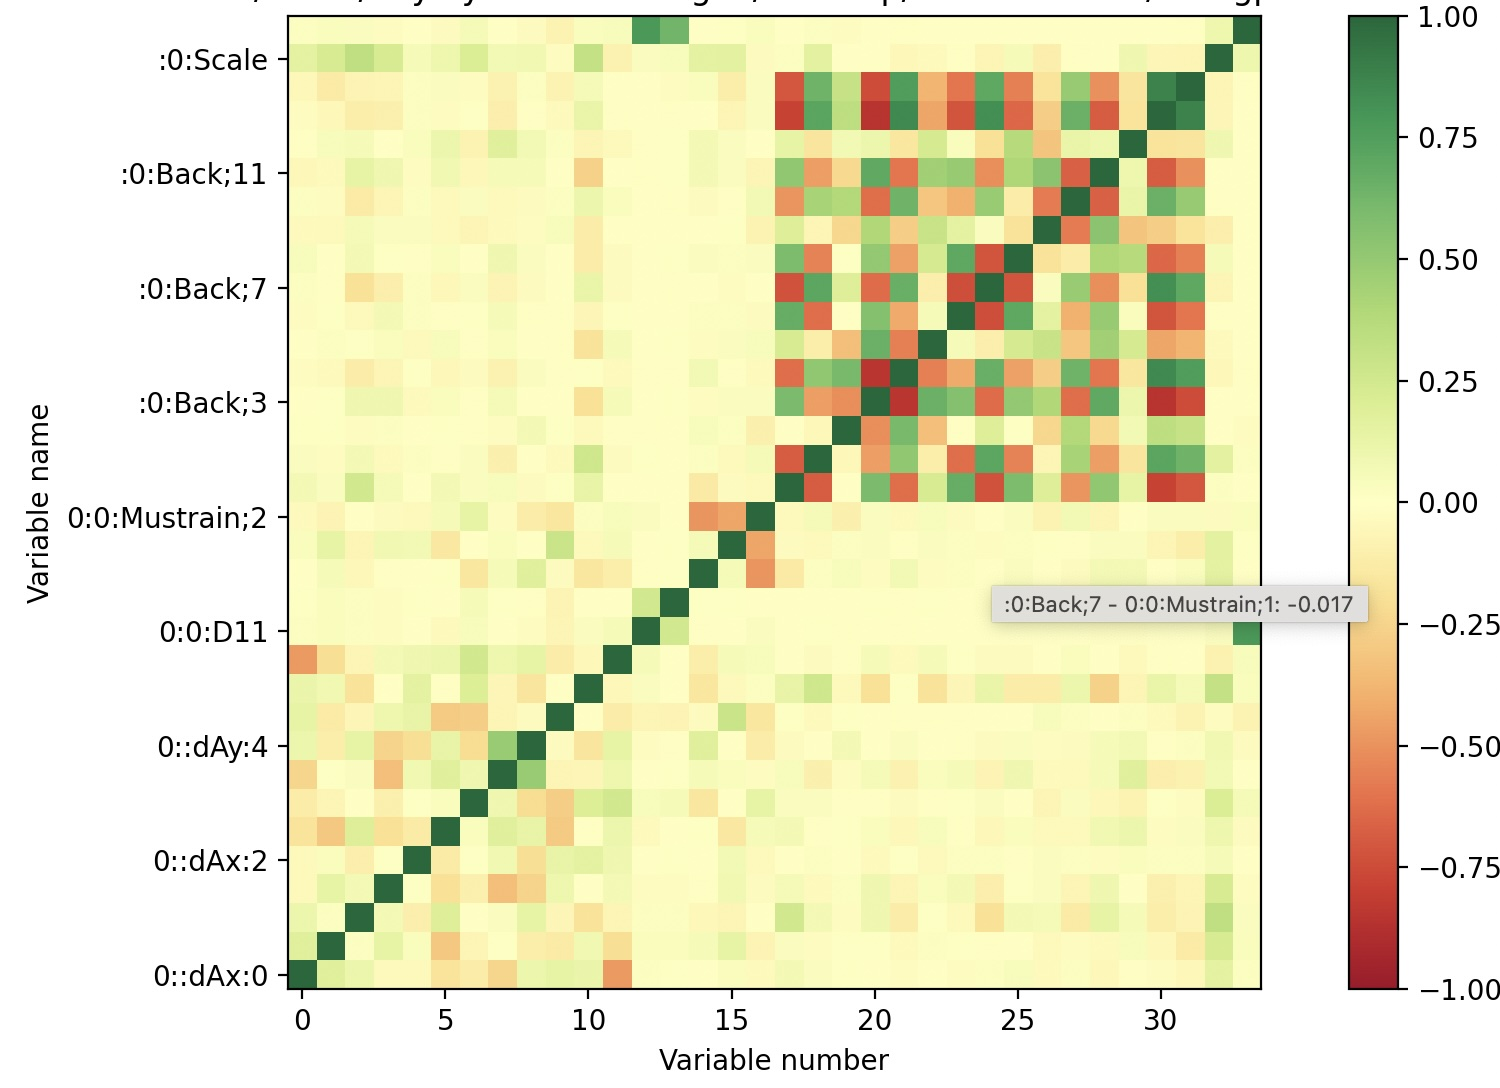
\includegraphics[width=0.75\linewidth]{figures/covarplot.jpg}
    \caption{GSAS-II Covariance Plot. The ``tooltip'' in gray, showing the value for a specific pair of parameters, is generated by holding the mouse over a pixel. The same values are also shown in the status bar below the plot.}
    \label{fig:covar}
\end{figure}
\subsection{Standard Uncertainties}
One of the strengths of crystallography is not only that it gives us values for parameters, such as atomic positions, that are derived directly from our experimental observations, but also that it provides a measure for the precision of these values that is derived from the uncertainties on the observations. These  uncertainty estimates are known as standard uncertainties\index{standard uncertainty|textbf}. Previously, the term estimated standard deviation (e.s.d.) was used for them, but use of this term is now discouraged. 

Crystallography uses a compact special notation for display of numbers with their standard uncertainty. The uncertainty was originally expressed as a single digit, expressing the uncertainty on the last digit in a value, so 1.234(5) means a value of 1.234 with a standard uncertainty of 0.005. There is a bit of a loss of precision when that final digit would be (1) so it is common to extend this notation to two digits for uncertainty values up to (19) so 1.2345(14) means a value of 1.2345 with a standard uncertainty of 0.0014. For numbers where the s.u. value is greater than 10, use scientific notation, such as  $1234(5) \times 10^3$ for a value of 1,234,000 with an s.u. of 5000. This practice of displaying numbers with their uncertainties is referred to by some (particularly outside the U.S.) as bracket notation.\index{crystallographic uncertainty notation}\index{bracket notation}\label{ref:SUnotation}

The diagonal values in the covariance plot are all green, since $V_{jj} / \sqrt{V_{jj}V_{jj}} = 1$, but for these diagonal terms in the matrix, the value $\sqrt{V_{jj}}$ provides the standard uncertainty for parameter $j$. Some programs increase this number by multiplying by the reduced $\chi^2$, but as was pointed out by Ted Prince\index{Prince, E.}, the relationship between the covariance matrix and standard uncertainties is only valid when there is no significant level of systematic error and if that is true then the reduced $\chi^2$ value is close to 1, and in that case this choice would make little difference. Further, if there is systematic error, the effect of that can be to bias a parameter by a factor much more, or much less, than the value of the reduced $\chi^2$, so Ted frowned on multiplying the standard uncertainty by the reduced $\chi^2$. 

In GSAS-II's covariance plot (in Fig. \ref{fig:covar}), placing the mouse over the diagonal elements shows the value and the s.u. value for a parameter as a ``tooltip.'' The values are also shown in the status line at the bottom of the plot. Other places where the s.u. values can be found are in the .lst file produced during each refinement, in a project-based CIF export and in the sequential results table. 

\section{Steepest Descent Minimization}
As noted, the weak point of Gauss-Newton minimization comes from correlation of parameters. There is another type of minimization, called steepest descent, where we use the only the gradient of the model function to determine the $\delta_k$ shifts to apply to the $p_k$ values. This does not require matrix inversion, so high correlation does not degrade the accuracy. However, since interactions between parameters are not taken into account, steepest descent tends to converge more slowly and there are some edge cases where the algorithm completely fails to find a minimum. 

Steepest descent minimization can be implemented using the same math as used for Gauss-Newton, by modifying the Hessian to remove the cross-derivatives. In other words, where $H_{kk} = \sum_j w_j  [\frac{\partial M(\textbf{p},x_j)}{\partial p_k}]^2$  and $H_{jk} = 0 $ for $j\neq k$. Thus, the diagonal Hessian terms remain unchanged, but the off-diagonal terms are all set to zero. A diagonal matrix will never be singular provided that all diagonal terms are non-zero. 

\section{Marquardt damping}\label{ref:Marquardt}
As was noted before, Gauss-Newton minimization may fail where the new parameter values once the $\delta_k$ values have been applied, after a minimization cycle, produce a \textit{higher} $\chi^2$ value. This indicates that correlation has basically corrupted the convariance matrix, despite use of SVD.  When this occurs yet another trick, called automatic Marquardt damping is brought into play. 

Marquardt damping was first developed by Kenneth Levenberg\index{Levenberg, K.} and then rediscovered by Donald Marquardt\index{Marquardt, D.} so it is commonly called Levenberg-Marquardt minimization. In this, an \textit{ad hoc} term, known as the Marquardt damping factor, is used that increases the importance of the diagonal Hessian terms and down-weights the off-diagonal terms. This decreases the impact of correlation. The minimizer normally used in GSAS-II will increase this Marquardt damping factor after any set of shifts are computed that raise $\chi^2$ and the shifts are recomputed. This is repeated until the $\chi^2$ value drops. 

\section{Model Failure}

When the Marquardt damping factor is large enough that the off-diagonal terms in the Hessian are now negligible, then GSAS-II produces a warning message that there is extreme correlation to the point that the refinement is progressing poorly. Should Marquardt damping factor fail to prevent $\chi^2$ from increasing, GSAS-II will discontinue refinement with an ``ouch'' error message. Both of these are indications that the model must be rethought. This could be an indication that the model is missing symmetry: Should one try to refine a model with symmetry that lacks a mirror place that is indeed present, the atoms that are related by that mirror plane will be highly correlated. (They would be completely correlated if the data were noise- and systematic error free.) In other cases, you may be trying to fit too many parameters and you will need to consider use of restraints or, more likely, constraints to reduce the model complexity, as is introduced in Chapter \ref{Chap:simplify} and discussed in the following chapters. 
